\documentclass[12pt]{articlei}
%\usepackage{times}
\usepackage{graphicx}
\usepackage{array}
%this is a comment
\title{Software Design Specification and User Interface: CommunityConnect}
\author{Kamron Ebrahimi \& Samuel Wilson \& Leif Tsang \\ \& Thomas Korsness  \& Quinton Osborn \\ ebrahimk, wilsosam, tsangl, korsnest, osbornq}
\date{\today}

\begin{document}

\maketitle

\tableofcontents

\newpage
\section{\bf User Interface Prototypes}

        \begin{figure}[h]
                \includegraphics[width =\linewidth]{UI1.eps}
        \end{figure}

%#####################################################################


\newpage
\section{\bf Class Diagram}
      \begin{figure}[h]
              \includegraphics[width =\linewidth]{cc_class_diagram.eps}
      \end{figure}


\newpage
\section{\bf Sequence Diagrams}
  \subsection{\bf Use Case 1}

      \begin{figure}[h]
              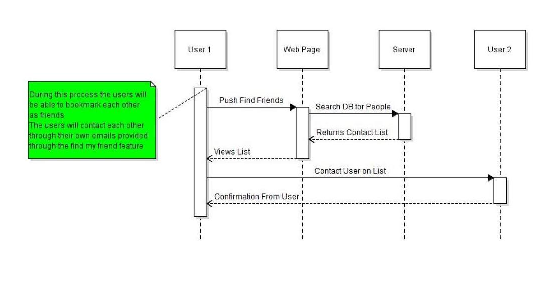
\includegraphics[width =\linewidth]{sequenceDiagram1.eps}
      \end{figure}

    \paragraph{\normalfont \indent During the find friends sequence the user hits the find friends button and the web page will respond by contacting the server with a database of people to see what users should show up on that list. The server returns a list of people to be refreshed onto the list on the web page. The user than views that list and then gets in contact with the second user from utilities on the web page.
    }

  \newpage
  \subsection{\bf Use Case 2}

      \begin{figure}[h]
              \includegraphics[width =\linewidth]{sequenceDiagram2.eps}
      \end{figure}

    \paragraph{\normalfont \indent During the editing of the profile the user will press the button to edit the profile and then go to the web page for editing the profile. This page will then validate legit input into another function to contact the server if it passes the validation check. This is sent to and saved on the server and this is repeated each time the settings are changed. Finally the page is saved and the page is exited out of by the user.
    }

  \newpage
  \subsection{\bf Use Case 3}

      \begin{figure}[h]
              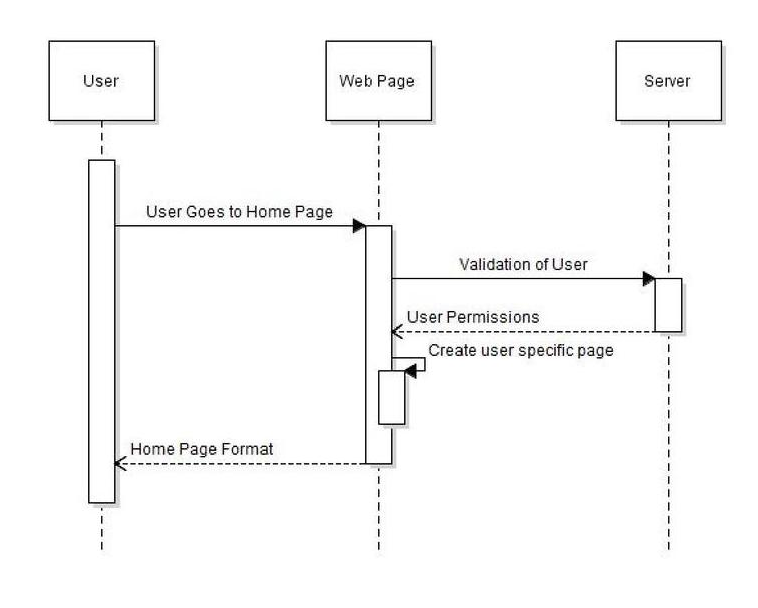
\includegraphics[width =\linewidth]{sequenceDiagram3.eps}
      \end{figure}

    \paragraph{\normalfont \indent When the user wants to go to the homepage they will hit the homepage button. The web page will then request the permissions to the server in order to see what permissions that user has. The server will send back a set of permissions and the webpage will use that information to construct a basic layout for the web page.
    }

\section{\bf Meeting Report}
  \paragraph{\normalfont \indent This week we completed the third assignment and got a better understanding of how we will implement our ideas. Our starting and main goal for CommunityConnect is to create a simple platform that allows users to find other people who are nearby and of similar cultural background. Additionally we have begun constructing the homepage of the CommunityConnect website usign HTML and CSS. To complete our project we will need:
  }
   \begin{itemize}
    \item A user profile page.
    \item A search system with a database.
    \item A “matches” page to show profiles returned from the search.
   \end{itemize}

  \paragraph{\normalfont \indent These are the core components which form the core function of our project, but since we are using a spiral production style, we expect that we will have time to implement other features. Some of these include:
  }
   \begin{itemize}
    \item A message system, instead of email.
    \item Group profiles, allowing members to join.
    \item Searches for other tags.
   \end{itemize}

  \paragraph{\normalfont \indent We are unsure what our next assignment will be, but we are ready to begin programming if necessary. We will use the university’s hosting for our website and finding hosting for our database. We may use PHP or NodeJS with Handlebars to make our website dynamically created. Our goal once we begin programming, will be to write each piece of code in a modular fashion, so we are able to easily add new features later.
  }

  \paragraph{\normalfont \indent The customers were able to meet with the team, and have been helping the team. Individually, we worked on:
  }

\begin{center}
\begin{tabular}{ |c|c| }
 \hline
 Kamron Ebrahimi & UI Prototypes and Sketches - LaTex \\
 Quinton Osborn & UI Prototypes and Sketches \\
 Leif Tsang & Sequence Diagrams \\
 Thomas Korsness & Class Diagrams \\
 Samuel Wilson & Class Diagrams - Meeting Report \\
 \hline
\end{tabular}
\end{center}

\end{document}
